\documentclass[11pt,a4paper,twocolumn]{article}

\usepackage{lipsum}
\usepackage{graphicx}
\usepackage{physics}

\begin{document}
\title{Elementar-Teilchen-Theorie Notizen}
\author{Maximilian Sackel}
\date{\today}
\maketitle

\section{Einleitung}
Elementarteilchenphysik bedeutet so viel wie die Suche nach neuen fudmanentalen
Naturgesetzen. 
Zur Beschreibung der Physik werden relativistische Quantenfelder genutzt.
Das wichtigste Modell in der Teilchenphysik ist das 'Standardmodell'.
\begin{figure}[h]
		\centering
		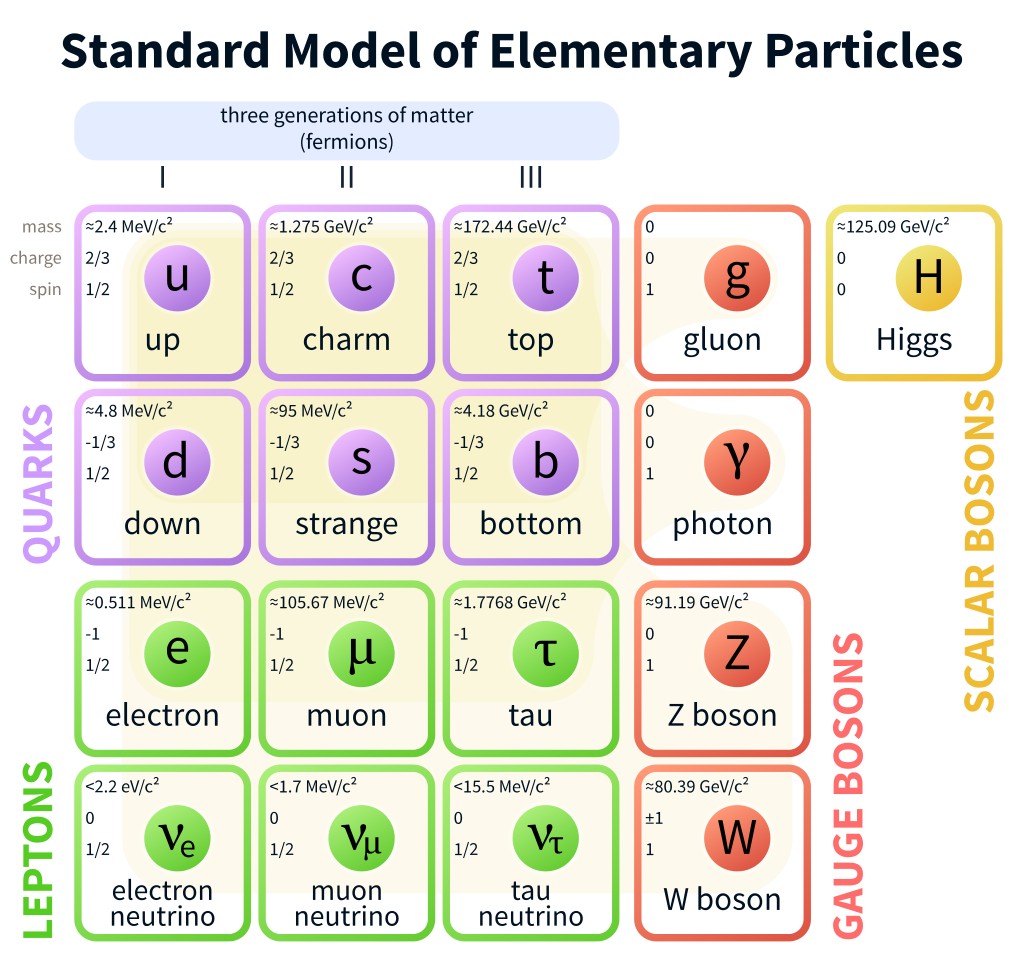
\includegraphics[width=0.4\textwidth]{./picture/Quark.png}
\end{figure}
Teilchenbahnen koennen aufgrund der QM nicht beobachtet werden. 
Die Anzahl an moeglichen Prozessen ist durch die Symmetrie eingeschraenkt.
(Raeummliche Trans./Impuls, zeitl. Trans./Energie, Drehung/Drehimpus, zufaell.
Sym...)

\subsection{Lorentztransformation}
Naturgesetze sind invariant unter Lorentztrafo.
\begin{equation}
		x \cdot y = \sum_{\mu \nu} x^{\mu} y^{nu} g_{\mu \nu}
\end{equation}
Dies laesst sich mittels eines Lorentzboost $x^{\mu} \to x'^{\mu} =
\Lambda^{\mu}_{\nu} x^{\nu} $ pruefen.
\begin{equation}
		x' \cdot y' = \Lambda^{\mu}_{\nu} x^{\nu} \cdot \Lambda^{\rho}_{\sigma}
		x^{\sigma} \cdot g_{\mu \nu} = x^{\nu} y^{\sigma} g_{\nu \sigma}
\end{equation}
Dazu muss der entsprechende metrische Tensor entsprechend $g_{\mu \nu}
\Lambda^{\mu}_{\rho} \Lambda^{\nu}_{\delta} \to g_{\rho \delta}$ tansformieren. 

\subsection{Kinematik von Streuprozessen}
Das Impulsquadrat ist allgemein in der ART eine invariante.
Fuer einen Prozess $p_a + p_b \to p_c + p_d$ laesst sich die Energieerhaltung
\begin{equation}
		p_a^0 + p_b^0 = p_c^0 + p_d^0 
\end{equation}
sowie Impulserhaltung 
\begin{equation}
		\vec{p_a} + \vec{p_b} = 0 = \vec{p_c} + \vec{p_d}
\end{equation}
im Schwerpunktsystem (CMS) definieren.
Dazu lassen sich die Lorentzinvarianten kinematischen Groessen/ 
Mandelstammvariablen definieren.
\begin{eqnarray}
		s = (p_a + p_b)^2 \\
		t = (p_a - p_c)^2 \\
		u = (p_a - p_d)^2
\end{eqnarray}
Diese sind linear abhaengig,
\begin{equation}
		(u + t + s) = \sum_i m_i
\end{equation}
sodass es nur zwei linear unabheanigige Variablen gibt.

\subsection{Integration auf der Massenschale}
Das Lorentzinvariante Integral einer beliebigen sklaraen Funktion $f(x)$ 
\begin{equation}
		\int d^4p \ \delta(p^2 -M^2) \theta(p^0) f(p)
\end{equation}
kann ueber die vierer Impulse $p^2 > 0, p^0 > 0$ kann geschrieben werden als
\begin{equation}
		\int d^3p \ \frac{f(\sqrt{\vec{p}^2 + M^2}, \vec{p})}{2\sqrt{\vec{p}^2
		+ M^2}}
\end{equation}
Zum beweis der Entwicklung wird die entwicklugn der Delta-Funktion genutzt wobei
$x_0$ die Nullstellen der Funktion $f$ sind.
\begin{equation}
		\delta(f(x)) = \frac{\delta(x-x_0)}{|f'(x_0)|}
\end{equation}

\section{Streutheorie}
\subsection{S-Matrix}
Man nehme an, der Hamiltonoperator bestehe aus einem Term $H_0$ welche ein 
beliebige Anzahl freier Teilchen beschreibt und einem Wechselwirkungsterm $V_0$
welcher verschwindet wenn die Teilche weit voneinader entfernt seien.
\begin{equation}
		H = H_0 + V
\end{equation}
Wir verwenden das Heisenbergbild und definieren ein- $\ket{\alpha, +}$ und
auslaufende $\ket{\beta, -}$ Zustaende als Eigenzustaende des Hamiltonians,
\begin{equation}
		H \ket{\alpha, \pm} = E_{\alpha} \ket{\alpha, \pm}
\end{equation}
so, dass fuer Messungen bei $t \to \pm \inf$ wie Eigenzustaende des Hamiltonians
$H_0$ fure freie Teilchen $\ket{\alpha}_0$ erscheinen.
Die Zustaende $\ket{\alpha, +}$ und $\ket{\beta, -}$ bilden eine Basis desselben
Hilbertraums. Daher koennen wir $\ket{\alpha, +}$ und $\ket{\beta, -}$
ausdruecken als 
\begin{equation}
		\ket{\alpha, +} = \int d\beta \ S_{\beta \alpha} \ket{\beta, -}
\end{equation}
Damit folgt $S_{\beta \alpha}$ ist also die Uebergangsamplitude fuer den Prozess
$\ket{\alpha, +} \to \ket{\beta, -}$.
\begin{equation}
		\bra{\alpha, +} \ket{\beta, -} =S_{\beta \alpha}
\end{equation}
Da die ein- und auslaufende Zustaende orthogonal sind ist die S-Matrix
Orthogonal.
Aufgrund zeitlicher und raeumlicher Translationsinvarianz sind Gesamtenergie und
Impuls im Streuprozess erhalten, daher schreiben wir
\begin{equation}
		S_{\beta \alpha} = \delta_{\alpha \beta} - 2 \pi i \delta(E_{\alpha} -
		E_{\beta})\delta^3(\vec{p_{\alpha}}-\vec{p_{\beta}}) M_{\beta \alpha}
\end{equation}
Die Uebergangswahrscheinlichkeit $P$ ist dann proportional zu $T$, wir
bezeichnen den Koeffizienten als differentielle Uebergangsrate.
\begin{equation}
		d\Gamma(\alpha \to \beta) = \frac{dP(\alpha \to \beta)}{T}
\end{equation}
Ueblicherweise misst man die Uerbergangsrate normiert auf den Fluss
$\Phi_{\alpha} = u_{\alpha}/V$ der einlaufenden Teilchen.
Der differnzielle Wirkungsquerschnitt $d\sigma$ ist definiert als
\begin{equation}
		d\sigma(\alpha \to \beta) = \frac{d\Gamma(\alpha \to
		\beta)}{\Phi_{\alpha}}
\end{equation}
\end{document}
